%%%%%%%%%%%%%%%%%%%%%%%%%%%%%%%%%%%%%%%%%%%%%%%%%%%%%%%%%%%%%%%%%%%%%%%%%%%%%%%
%% StuPro B, "Programmierumgebung Offener Antrieb" (POA)
%% Handbuch Tutorial
%% $Id: tutorial.tex,v 1.4 2004/03/19 00:08:54 neco Exp $
%% Achtung: Diese Datei wird in das Handbuch inkludiert!
%%%%%%%%%%%%%%%%%%%%%%%%%%%%%%%%%%%%%%%%%%%%%%%%%%%%%%%%%%%%%%%%%%%%%%%%%%%%%%%

\chapter {Tutorial}
Um dem Benutzer einen leichten Einstieg in POA zu verschaffen, wird in diesem Kapitel ein POA-Projekt anhand eines einfachen Regelkreises f"ur eine Antriebsregelung realisiert. Die Abbildung 4.1 gibt alle n"otigen Daten f"ur das Projekt wieder.
\begin{figure}[htbp]

\begin{center}

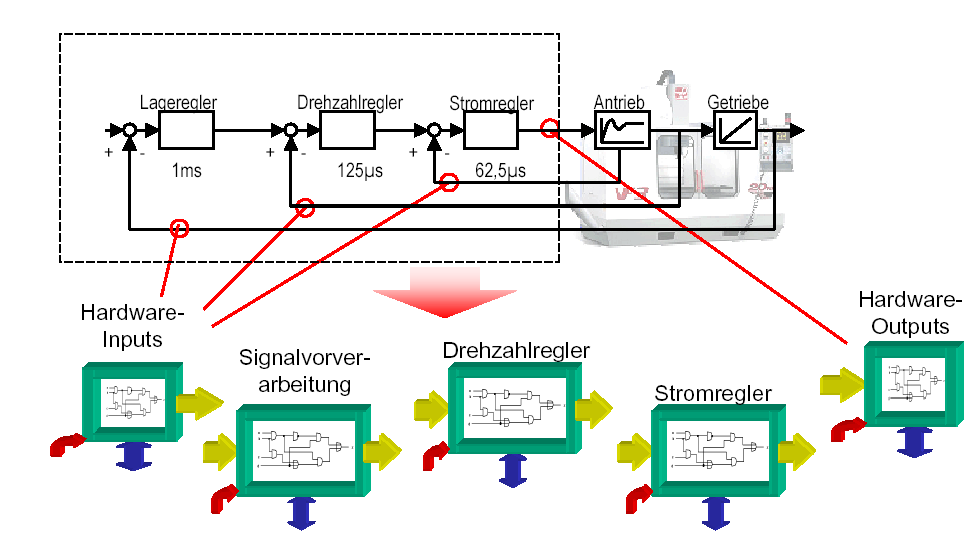
\includegraphics[width=15cm]{Beispielsprojekt}
\caption{Beispielsprojekt}\label{test}
\end{center}

\end{figure}
\newline
Standard Regelkreis:
\begin{itemize}
	\item Lageregler: Eing"ange {\itshape xSoll[32], xIst[32]} und Ausgang {\itshape nSoll[32]}
	\item Drehzahlregler: Eing"ange {\itshape nSoll[32], nIst[32]} und Ausgang {\itshape iSoll[10]}
	\item Stromregler: Eing"ange {\itshape iSoll[10], iIst[10]} und Ausgang {\itshape stell[10]}
\end{itemize}

Zus"atzlich:
\begin{itemize}
	\item Signalvorverabeitung: Eing"ange {\itshape xIst-raw, nIst-raw, iIst-raw} und Ausg"ange {\itshape xIst[32], nIst[32], iIst[10]}
	\item HardwareInputs: Ausg"ange {\itshape xSoll[32], xIst-raw, nIst-raw, iIst-raw}
	\item HardwareOutput: Eingang {\itshape stell[10]}
\end{itemize}
Die Zahlen in den eckigen Klammern geben die Bitbreite an.
\par

\section {Beispielprojekt  anlegen}
Bevor man mit dem Layout f"ur den Antriebsregler anfangen kann, muss zun"achts einmal das Projekt angelegt werden. Dazu muss man folgenderma"sen vorgehen:
\begin{enumerate}
	\item In der Men"uleiste {\bf Project} den Eintrag {\bf New} ausw"ahlen.
	\item Im Dialog {\bf Select/Create project directory} den gew"unschten Pfad angeben.
	\item Den Button {\bf Create New Directory} anklicken.
	\item Name des Projekt eingeben und mit Return best"atigen.
	\item Den neu erzeugten Ordner anw"ahlen und den Button {\bf Open} dr"ucken.
	\item Die Datei {\bf project.xlm} anw"ahlen und den Button {\bf Open} dr"ucken.
\end{enumerate}
Nach dem Anlegen und "offnen des neuen Projekt wird das Arbeitsfenster mit einem leeren Layout ge"offnet.
\section{Funktionsbl"ocke erzeugen und konfigurieren}
Zur Realisierung des Antriebreglers ben"otigt man verschiedene Typen von Bl"ocken und zwar:
\begin{itemize}
	\item 2 I/O-Bl"ocke, einen f"ur HardwareInput und einen f"ur HardwareOutput
	\item 3 CPU-Bl"ocke f"ur Signalverarbeitung, Lageregler und Drehzahlregler
	\item 1 Core-Block f"ur Stromregler
\end{itemize}
\subsection{HardwareInput und HardwareOutput}
HardwareInput und HardwareOutput bilden die Schnittstelle nach Au"sen. Daher werden I/O-Bl"ocke verwendet. Die ankommenden Signale werden "uber den HardwareInput-Block an den Singalverarbeitungsblock weitergeleitet. Signale, die nach Au"sen weitergeleitet werden m"ussen, kommen in den HardwareOutput-Block. Als erstes wird der HardwareInput erzeugt und konfiguriert:
\begin{enumerate}
	\item Einen I/O-Block aus der Blockbiliothek per Drag'n Drop ziehen, d.h. mit dem Mauszeiger den Block ankilcken, die Maustaste dabei gedr"uckt lassen, den Block ins Arbeitsfenster ziehen und die Maustaste wieder loslassen.
	\item Im Dialog {\bf Block configuration} als erstes den Namen {\itshape "'HardwareInput"'} eingeben
	\item Unter {\bf Description} den Block beschreiben {\itshape "'..."uber diesen Inputblock werden die Signale weitergeleitet..."'}.
	\item Den Offset Eintrag auf {\itshape "'Auto (0 ns)"'} lassen.
	\item Unter {\bf Clock} den Takt f"ur den HardwareInput-Block angeben, d.h. standardm"a"sig {\itshape "'0 ns"'} f"ur I/O-Bl"ocke.
	\item Unter {\bf Runtime} den Eintrag auf 1 lassen.
	\item In der Pintabelle die Pins f"ur die 4 Ausg"ange erzeugen und konfigurieren:
		\begin{itemize}
			\item Zum Erzeugen von Pins, die Pinkategorie ausw"ahlen und den Button {\bf New} dr"ucken.
			\item In der Spalte {\bf Name} Pinnamen, d.h. die Bezeichnungen f"ur die Ausg"ange angeben.
			\item In der Spalte {\bf Bits} die Bitbreiten [Anzahl der Bits] der Ausgangssignale angeben.
			\item In der Spalte {\bf Address} eine Speicheradresse angeben.
			\item Mit den Pfeiltasten kann die Reihenfolge der Pins ge"andert werden.
		\end{itemize}
	\item Nach der Konfiguration aller Pins den {\bf OK} Button dr"ucken.
\end{enumerate}
F"ur die Erstellung und Konfiguration des HardwareOutput-Blocks muss man dem entsprechend vorgehen.

\subsection{Signalverarbeitung, Lageregler und Drehzahlregler}
Diese Elemente der Antriebsregelung sind frei programmierbar. Daher werden sie durch CPU-Bl"ocke realisiert. Die Erzeugung und Konfiguration dieser Bl"ocke entspricht weitestgehend den oben beschriebenen Bl"ocken. Die Konfiguration dieser Bl"ocke bietet einige weitere M"oglichkeiten:
\begin{enumerate}
	\item Im Feld {\bf ID} muss der CPU eine eindeutige Identifikationsnummer gegeben werden.
	\item Zum Erzeugen des CPU-Programmcodes den Button {\bf Edit Code} dr"ucken.
	\item Zum Kompilieren des CPU-Programmcodes den Button {\bf Compile} dr"ucken.
\end{enumerate}

\subsection{Stromregler}
Der Stromregler besitzt eine festgelegte Logik und Laufzeit. Daher wird er duch ein Core-Block realisiert.


\section{Funktionsbl"ocke verbinden}
Nachdem alle erforderlichen Bl"ocke erzeugt und weitestgehend konfiguriert worden sind, m"ussen die Bl"ocke miteinander verbunden werden. Zum Verbinden von zwei Bl"ocken muss mit der Maustaste den Ausgangspin (xSoll) des einen Blocks anklicken, die Taste gedr"uckt halten und mit dem Cursor an den Eingangspin (xSoll) des Anderen andocken. Nach der Verbindung aller Pins erh"alt man eine Vernetzung etwa wie in Abb. 4.2.
\begin{figure}[htbp]

\begin{center}

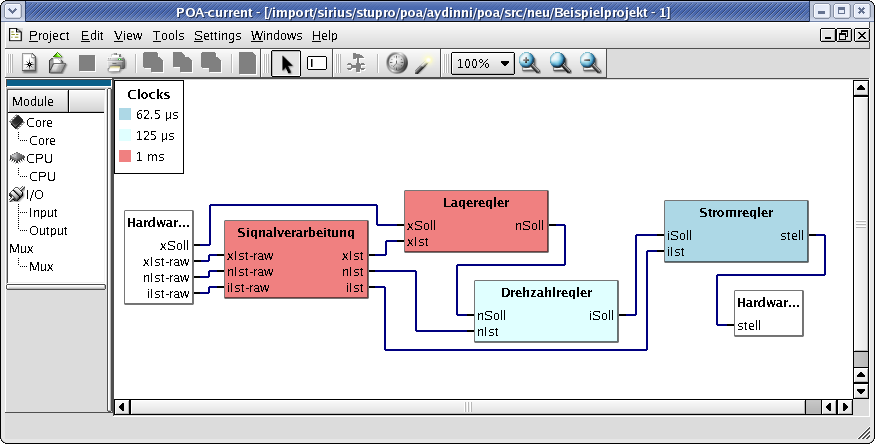
\includegraphics[width=15cm]{Bspprojekt1}
\caption{Beispielsprojekt Layout}\label{test}
\end{center}

\end{figure}
